%! Unidad 8 — Física nuclear (teoría, actividades resueltas y prácticas)
%! Fuente: Fuentes/Tema_8.pdf (reescrito; datos de las actividades cambiados y recalculados)

\section*{Para empezar: unas placas veladas}
\addcontentsline{toc}{section}{Para empezar: unas placas veladas}

En 1896, Henri Becquerel guardó en un cajón unas sales de uranio junto a unas placas fotográficas envueltas en papel negro.
Al revelarlas, descubrió que se habían velado: las sales emitían, sin que nada las estimulara, una radiación invisible capaz de
atravesar el papel. Marie y Pierre Curie llamaron a este fenómeno \emph{radiactividad} y descubrieron dos nuevos elementos, el
polonio y el radio. Aquellas placas veladas fueron la primera señal de que el núcleo de los átomos guarda una energía enorme: la
que hace brillar al Sol, la que se aprovecha en las centrales nucleares y la que permite datar fósiles o tratar tumores. En esta
unidad estudiaremos cómo es el núcleo, por qué es estable o inestable y cómo se transforma.

\section{El núcleo atómico}\label{sec:nuc-nucleo}

En 1911, Ernest Rutherford bombardeó una lámina de oro muy fina con partículas alfa. Casi todas la atravesaban sin desviarse,
pero unas pocas rebotaban. Dedujo que el átomo es casi vacío y que su carga positiva y casi toda su masa están concentradas en una
región diminuta: el \rojon{núcleo}. Hoy sabemos que el núcleo está formado por dos tipos de partículas, los \azuln{nucleones}:
\begin{itemize}
    \item el \textbf{protón}, con carga \(+e = \qty{1.6e-19}{\coulomb}\) y masa \(m_p = \qty{1.6726e-27}{\kg} = \qty{1.0073}{u}\);
    \item el \textbf{neutrón}, sin carga y con una masa algo mayor, \(m_n = \qty{1.6749e-27}{\kg} = \qty{1.0087}{u}\).
\end{itemize}
Los electrones, casi 2000 veces más ligeros, forman la corteza.

\begin{figure}[H]
    \centering
    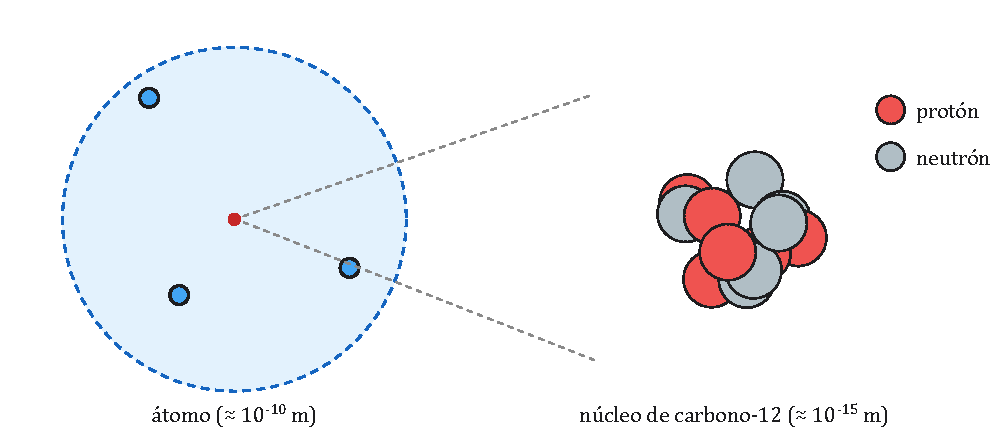
\includegraphics[width=0.75\linewidth]{images/UD8/nucleo}
    \caption{Si el átomo fuera un estadio de fútbol, el núcleo sería una canica en el centro (dibujo sin escala).}
    \label{fig:nuc-nucleo}
\end{figure}

\paragraph{Número atómico y número másico.} El \azuln{número atómico} \(Z\) es el número de protones; identifica al elemento. El
\azuln{número másico} \(A\) es el número total de nucleones, \(A = Z + N\), donde \(N\) es el número de neutrones. Un núcleo (o
\emph{nucleido}) se representa como \(\ch{^{A}_{Z}X}\): por ejemplo, \(\ch{^{235}_{92}U}\) tiene 92 protones y 143 neutrones.
\begin{itemize}
    \item \textbf{Isótopos}: mismo \(Z\) y distinto \(A\) (\ch{^{12}_{6}C} y \ch{^{14}_{6}C}). Son el mismo elemento.
    \item \textbf{Isóbaros}: mismo \(A\) y distinto \(Z\) (\ch{^{14}_{6}C} y \ch{^{14}_{7}N}).
    \item \textbf{Isótonos}: mismo número de neutrones (\ch{^{13}_{6}C} y \ch{^{14}_{7}N}).
\end{itemize}
La masa atómica de un elemento es la media ponderada de las masas de sus isótopos según su abundancia, por eso casi nunca es entera.

\paragraph{Unidad de masa atómica.} Es la doceava parte de la masa de un átomo de \ch{^{12}C}:
\(\qty{1}{u} = \dfrac{\qty{12e-3}{\kg\per\mol}}{12\cdot\qty{6.022e23}{\per\mol}} = \qty{1.66e-27}{\kg}\).

\paragraph{Tamaño del núcleo.} Los átomos miden unos \qty{e-10}{\m} y los núcleos, entre \qty{e-15}{\m} y \qty{e-14}{\m}. El radio
de un núcleo crece con la raíz cúbica de su número másico:
\begin{centeredequation}
    \boxed{R = r_0\,A^{1/3}} \qquad r_0 = \qty{1.2e-15}{\m} = \qty{1.2}{\femto\m} \label{eq:nuc-radio}
\end{centeredequation}
Como el volumen es proporcional a \(R^3\), es proporcional a \(A\): todos los núcleos tienen prácticamente la misma densidad, unos
\qty{2.3e17}{\kg\per\m\cubed}. Una cucharadita de materia nuclear pesaría más de mil millones de toneladas.

\begin{exercise}
    Calcula el radio, el volumen y la densidad de un núcleo de \ch{^{16}O}.
    \begin{solu}
        \(R = 1{,}2\cdot 10^{-15}\cdot 16^{1/3} = \textcolor{red}{\qty{3.02e-15}{\m}}\); \(V = \tfrac{4}{3}\pi R^3 = \textcolor{red}{\qty{1.16e-43}{\m\cubed}}\);
        \(\rho = \dfrac{16\cdot 1{,}66\cdot 10^{-27}}{1{,}16\cdot 10^{-43}} = \textcolor{red}{\qty{2.3e17}{\kg\per\m\cubed}}\).
    \end{solu}
\end{exercise}

\section{Las fuerzas nucleares}\label{sec:nuc-fuerzas}

Los protones del núcleo, muy próximos y con carga del mismo signo, se repelen con fuerzas eléctricas enormes. La gravedad entre
ellos es despreciable. Para que el núcleo exista tiene que haber otra interacción, atractiva y mucho más intensa: la
\rojon{interacción nuclear fuerte}. Sus características son:
\begin{itemize}
    \item Es la más intensa de las interacciones conocidas (unas 100 veces más que la eléctrica a esas distancias).
    \item Es de \textbf{muy corto alcance} (unos \qty{e-15}{\m}): cada nucleón solo atrae a sus vecinos inmediatos (\azuln{saturación}).
    \item Es \textbf{independiente de la carga}: actúa igual entre protón y protón, neutrón y neutrón, o protón y neutrón.
\end{itemize}
Los neutrones contribuyen a la atracción nuclear sin añadir repulsión eléctrica: son el «pegamento» que estabiliza los núcleos.

\section{Energía de enlace}\label{sec:nuc-enlace}

\subsection{Equivalencia entre masa y energía}\label{subsec:nuc-masa-energia}

Una de las consecuencias de la relatividad especial es que la masa es una forma de energía:
\begin{centeredequation}
    \boxed{E = m\,c^2} \label{eq:nuc-einstein}
\end{centeredequation}
En los procesos químicos los cambios de masa son imperceptibles, pero en los nucleares no: al fisionarse un gramo de uranio-235
desaparece aproximadamente un miligramo de masa, que se convierte en tanta energía como la combustión de unas tres toneladas de
carbón. Los principios de conservación de la masa y de la energía se funden en uno solo: \emph{en un sistema aislado, la suma de la
energía y del equivalente energético de la masa se conserva}.

\begin{exercise}
    Calcula, en MeV, la energía equivalente a \qty{1}{u}.
    \begin{solu}
        \(E = mc^2 = 1{,}66\cdot 10^{-27}\cdot(3\cdot 10^8)^2 = \qty{1.494e-10}{\joule} = \dfrac{1{,}494\cdot 10^{-10}}{1{,}6\cdot 10^{-13}} = \textcolor{red}{\qty{934}{\mega\electronvolt}}\).
        \textcolor{blue}{(Con valores más precisos de las constantes, \(\qty{1}{u} \equiv \qty{931.5}{\mega\electronvolt}\), que es el que usaremos.)}
    \end{solu}
\end{exercise}

\subsection{Defecto de masa y energía de enlace}\label{subsec:nuc-defecto}

Al medir con precisión la masa de un núcleo se comprueba que es \textbf{menor} que la suma de las masas de sus nucleones por
separado. La diferencia es el \rojon{defecto de masa}:
\begin{centeredequation}
    \Delta m = Z\,m_p + (A - Z)\,m_n - m_{\text{núcleo}} \label{eq:nuc-defecto}
\end{centeredequation}
Esa masa «perdida» es la energía que se libera al formarse el núcleo, la \rojon{energía de enlace}, que es también la energía mínima
necesaria para separarlo en sus nucleones:
\begin{centeredequation}
    \boxed{E_e = \Delta m\,c^2} \qquad\quad \Delta m\ (\text{en u})\ \Rightarrow\ E_e\ (\text{en MeV}) = 931{,}5\,\Delta m \label{eq:nuc-enlace}
\end{centeredequation}
Si se usa la masa del \emph{átomo} en lugar de la del núcleo, hay que tomar la del átomo de hidrógeno (\qty{1.0078}{u}) en lugar de la
del protón, para que los electrones se cancelen.

\paragraph{Energía de enlace por nucleón.} La estabilidad de un núcleo no la indica su energía de enlace total, sino la
\azuln{energía de enlace por nucleón}, \(E_e/A\): la energía media necesaria para arrancar un nucleón. Cuanto mayor es, más estable
es el núcleo (figura~\ref{fig:nuc-curva}). Crece rápidamente en los núcleos ligeros, alcanza un máximo de unos \qty{8.8}{\mega\electronvolt}
hacia el hierro-56 y desciende suavemente en los pesados.

\begin{figure}[H]
    \centering
    \begin{tikzpicture}
        \begin{axis}[fisica, width=0.8\linewidth, height=5.6cm, xmin=0, xmax=250, ymin=0, ymax=10,
            xlabel={\(A\)}, ylabel={\(E_e/A\) (\unit{\mega\electronvolt})}, xtick={50,100,150,200,250}, ytick={2,4,6,8}, samples=200]
            % fórmula semiempírica de Weizsäcker (sin término de apareamiento)
            \addplot[domain=12:240, very thick, ocre] {15.75 - 17.8/x^(1/3) - 0.711*(x/(1.98+0.015*x^(2/3)))^2/x^(4/3) - 23.7*((x-2*(x/(1.98+0.015*x^(2/3))))/x)^2};
            \addplot[only marks, mark=*, mark size=1.8pt, blue] coordinates {(2,1.11) (3,2.83) (4,7.07) (6,5.33) (7,5.61) (12,7.68) (16,7.98) (20,8.03) (56,8.79) (120,8.5) (209,7.85) (235,7.59) (238,7.57)};
            \node[font=\scriptsize, anchor=west] at (axis cs:5,7.3) {\ch{^4He}};
            \node[font=\scriptsize, anchor=south] at (axis cs:56,8.9) {\ch{^{56}Fe}};
            \node[font=\scriptsize, anchor=north] at (axis cs:235,7.4) {\ch{^{235}U}};
            \node[font=\scriptsize, anchor=west] at (axis cs:4,1.1) {\ch{^2H}};
            \draw[->, thick, red] (axis cs:20,3) -- node[below, font=\scriptsize]{fusión} (axis cs:50,3);
            \draw[->, thick, red] (axis cs:230,5) -- node[below, font=\scriptsize]{fisión} (axis cs:150,5);
        \end{axis}
    \end{tikzpicture}
    \caption{Energía de enlace por nucleón (la curva, calculada con la fórmula semiempírica; los puntos, valores medidos). Se libera
    energía al fusionar núcleos ligeros o al fisionar núcleos pesados: en los dos casos se avanza hacia el máximo.}
    \label{fig:nuc-curva}
\end{figure}

\begin{remark}
    Esta curva explica las dos fuentes de energía nuclear: al \textbf{fusionar} núcleos ligeros o al \textbf{fisionar} núcleos pesados
    se obtienen núcleos con mayor energía de enlace por nucleón, más estables, y la diferencia se libera.
\end{remark}

\begin{exercise}
    Calcula el defecto de masa, la energía de enlace y la energía de enlace por nucleón del \ch{^{23}_{11}Na}, cuya masa atómica es
    \qty{22.98977}{u} (\(m_{\text{H}} = \qty{1.0078}{u}\), \(m_n = \qty{1.0087}{u}\)).
    \begin{solu}
        \(\Delta m = 11\cdot 1{,}0078 + 12\cdot 1{,}0087 - 22{,}98977 = \textcolor{red}{\qty{0.2004}{u}}\);
        \(E_e = 0{,}2004\cdot 931{,}5 = \textcolor{red}{\qty{186.7}{\mega\electronvolt}}\);
        \(\dfrac{E_e}{A} = \textcolor{red}{\qty{8.12}{\mega\electronvolt}}\) \textcolor{blue}{por nucleón.}
    \end{solu}
\end{exercise}

\subsection{Estabilidad nuclear}\label{subsec:nuc-estabilidad}

De los más de 3000 nucleidos conocidos, solo unos 250 son estables. Si se representa el número de neutrones frente al de protones de
los núcleos estables (figura~\ref{fig:nuc-estabilidad}), se agrupan en una franja, la \azuln{banda de estabilidad}. Los núcleos ligeros
estables tienen \(N \approx Z\); los pesados necesitan cada vez más neutrones (hasta \(N/Z \approx 1{,}5\)) para compensar la repulsión
eléctrica, que crece más deprisa que la atracción nuclear. Por encima de \(Z = 83\) (bismuto) no hay núcleos estables. Los núcleos que
quedan fuera de la banda son radiactivos: se transforman hasta llegar a ella.

\begin{figure}[H]
    \centering
    \begin{tikzpicture}
        \begin{axis}[fisica, width=0.62\linewidth, height=5.6cm, xmin=0, xmax=95, ymin=0, ymax=150,
            xlabel={\(Z\)}, ylabel={\(N\)}, xtick={20,40,60,80}, ytick={40,80,120}, samples=100]
            \addplot[name path=sup, draw=none, domain=1:83] {x + 0.0075*x^2 + 2 + 0.06*x};
            \addplot[name path=inf, draw=none, domain=1:83] {x + 0.0075*x^2 - 1 + 0.01*x};
            \addplot[ocre!40] fill between[of=sup and inf];
            \addplot[domain=0:90, thick, dashed, gray] {x};
            \node[font=\scriptsize, gray, anchor=west] at (axis cs:62,58) {\(N = Z\)};
            \node[font=\scriptsize, anchor=east] at (axis cs:60,110) {banda de estabilidad};
            \node[font=\scriptsize, red, anchor=west] at (axis cs:30,85) {exceso de \(n\): \(\beta^-\)};
            \node[font=\scriptsize, blue, anchor=west] at (axis cs:55,45) {exceso de \(p\): \(\beta^+\)};
            \node[font=\scriptsize, anchor=west] at (axis cs:83,135) {\(\alpha\)};
        \end{axis}
    \end{tikzpicture}
    \caption{Banda de estabilidad. Los núcleos con demasiados neutrones emiten \(\beta^-\); los que tienen demasiados protones,
    \(\beta^+\); los muy pesados, \(\alpha\).}
    \label{fig:nuc-estabilidad}
\end{figure}

\section{La radiactividad}\label{sec:nuc-radiactividad}

La \rojon{radiactividad} es la emisión espontánea de partículas o de radiación por parte de núcleos inestables, que así se transforman
en otros más estables. No depende de la temperatura, la presión ni el estado químico: es un fenómeno puramente nuclear.

\subsection{Tipos de radiación}\label{subsec:nuc-tipos}

Si se hace pasar la radiación de una muestra radiactiva por un campo magnético, se separa en tres componentes
(figura~\ref{fig:nuc-radiaciones}):
\begin{itemize}
    \item \textbf{Radiación alfa} (\(\alpha\)): núcleos de helio, \(\ch{^4_2He}\), con carga \(+2e\). Muy ionizante y poco penetrante:
    la detiene una hoja de papel o unos centímetros de aire.
    \item \textbf{Radiación beta} (\(\beta^-\)): electrones rápidos, que \emph{no} estaban en la corteza: se crean en el núcleo al
    transformarse un neutrón en un protón. Más penetrante: la detienen unos milímetros de aluminio.
    \item \textbf{Radiación gamma} (\(\gamma\)): ondas electromagnéticas de muy alta frecuencia (fotones muy energéticos), sin carga ni
    masa. Muy penetrante: hacen falta varios centímetros de plomo o metros de hormigón para atenuarla.
\end{itemize}

\begin{figure}[H]
    \centering
    \begin{minipage}[b]{0.48\linewidth}
        \centering
        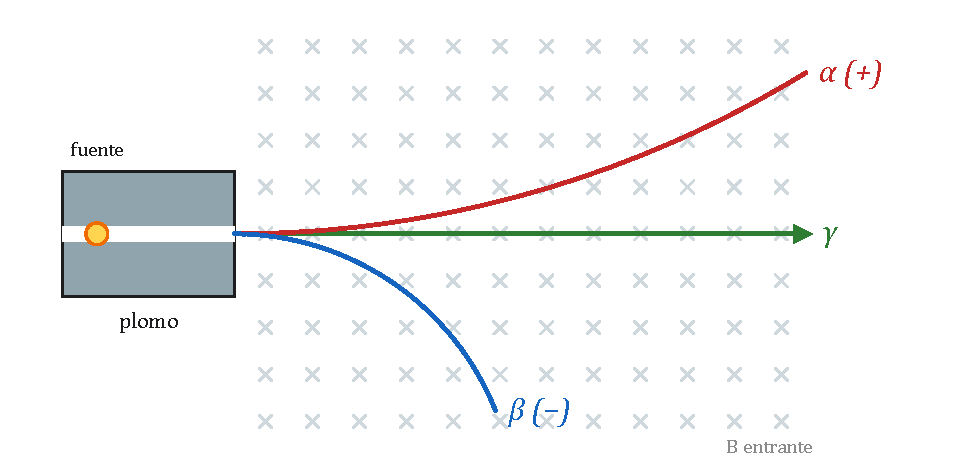
\includegraphics[width=\linewidth]{images/UD8/radiaciones}
    \end{minipage}\hfill
    \begin{minipage}[b]{0.48\linewidth}
        \centering
        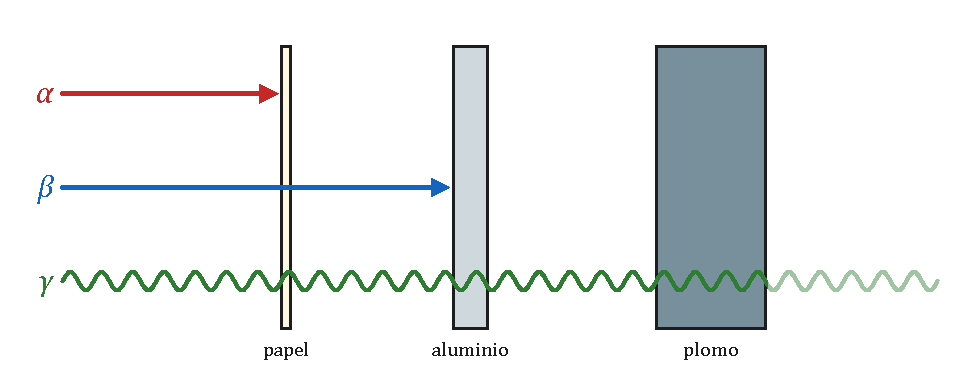
\includegraphics[width=\linewidth]{images/UD8/penetracion}
    \end{minipage}
    \caption{Izquierda: desviación de las radiaciones en un campo magnético (las \(\alpha\), mucho más pesadas, se curvan menos).
    Derecha: poder de penetración.}
    \label{fig:nuc-radiaciones}
\end{figure}

\subsection{Leyes de los desplazamientos radiactivos}\label{subsec:nuc-soddy}

En toda reacción nuclear se conservan la carga (la suma de los \(Z\)) y el número de nucleones (la suma de los \(A\)). De ahí salen las
\rojon{leyes de Soddy y Fajans}:
\begin{itemize}
    \item \textbf{Emisión \(\alpha\)}: el número atómico disminuye en 2 y el másico en 4. El elemento retrocede dos lugares en la tabla
    periódica:
    \[ \ch{^{A}_{Z}X -> ^{A-4}_{Z-2}Y + ^{4}_{2}He} \qquad\text{p. ej.}\quad \ch{^{238}_{92}U -> ^{234}_{90}Th + ^4_2He} \]
    \item \textbf{Emisión \(\beta^-\)}: un neutrón se transforma en un protón, un electrón y un antineutrino. \(Z\) aumenta en 1 y \(A\) no
    cambia; el elemento avanza un lugar:
    \[ \ch{^{A}_{Z}X -> ^{A}_{Z+1}Y + ^{0}_{-1}e} + \bar{\nu} \qquad\text{p. ej.}\quad \ch{^{14}_6C -> ^{14}_7N + ^0_{-1}e} \]
    \item \textbf{Emisión \(\beta^+\)} (radiactividad artificial): un protón se transforma en un neutrón, un positrón y un neutrino. \(Z\)
    disminuye en 1.
    \item \textbf{Emisión \(\gamma\)}: el núcleo pasa de un estado excitado a otro de menor energía; no cambian ni \(Z\) ni \(A\).
    Suele acompañar a las otras emisiones.
\end{itemize}

\begin{exercise}
    Completa las reacciones nucleares:
    \begin{enumerate}[label=\letraminuscula]
        \item \(\ch{^{14}_7N + ^4_2He -> X + ^{17}_8O}\)
        \item \(\ch{^{9}_4Be + X -> ^{12}_6C + ^1_0n}\)
        \item \(\ch{^{226}_{88}Ra -> X + ^4_2He}\)
    \end{enumerate}
    \begin{solu}
        \textcolor{blue}{Se igualan las sumas de \(A\) y de \(Z\) en los dos miembros.}
        \begin{enumerate}[label=\letraminuscula]
            \item \(A = 18 - 17 = 1\), \(Z = 9 - 8 = 1\): \(\textcolor{red}{\ch{X} = \ch{^1_1H}}\) (un protón; es la primera transmutación artificial, de Rutherford).
            \item \(A = 13 - 9 = 4\), \(Z = 6 - 4 = 2\): \(\textcolor{red}{\ch{X} = \ch{^4_2He}}\) (así descubrió Chadwick el neutrón).
            \item \(A = 222\), \(Z = 86\): \(\textcolor{red}{\ch{X} = \ch{^{222}_{86}Rn}}\).
        \end{enumerate}
    \end{solu}
\end{exercise}

\subsection{Ley de la desintegración radiactiva}\label{subsec:nuc-ley}

La desintegración es un proceso \textbf{aleatorio}: no se puede saber cuándo se desintegrará un núcleo concreto, solo la probabilidad de
que lo haga. En una muestra con \(N\) núcleos, el número que se desintegra en un tiempo \(dt\) es proporcional a \(N\) y a \(dt\):
\begin{equation*}
    dN = -\lambda\,N\,dt \qquad\Rightarrow\qquad \int_{N_0}^{N}\dfrac{dN}{N} = -\lambda\int_0^t dt \qquad\Rightarrow\qquad \ln\dfrac{N}{N_0} = -\lambda t
\end{equation*}
\begin{centeredequation}
    \boxed{N = N_0\,e^{-\lambda t}} \label{eq:nuc-ley}
\end{centeredequation}
\(\lambda\) es la \azuln{constante de desintegración} (\unit{\per\second}), característica de cada nucleido: es la probabilidad de que un
núcleo se desintegre por unidad de tiempo. La misma ley vale para la masa de la muestra, \(m = m_0 e^{-\lambda t}\).

\paragraph{Actividad.} La \rojon{actividad} es el número de desintegraciones por unidad de tiempo:
\begin{centeredequation}
    \boxed{A = \left|\dfrac{dN}{dt}\right| = \lambda\,N} \qquad\Rightarrow\qquad A = A_0\,e^{-\lambda t} \label{eq:nuc-actividad}
\end{centeredequation}
Su unidad en el SI es el \azuln{becquerel} (\(\qty{1}{\becquerel}\) = una desintegración por segundo). También se usa el
\emph{curio}: \(\qty{1}{Ci} = \qty{3.7e10}{\becquerel}\) (la actividad de un gramo de radio).

\paragraph{Período de semidesintegración y vida media.} El \rojon{período de semidesintegración} \(T_{1/2}\) es el tiempo que tarda en
desintegrarse la mitad de los núcleos. Haciendo \(N = N_0/2\):
\begin{centeredequation}
    \dfrac{1}{2} = e^{-\lambda T_{1/2}} \qquad\Rightarrow\qquad \boxed{T_{1/2} = \dfrac{\ln 2}{\lambda}} \label{eq:nuc-semi}
\end{centeredequation}
Al cabo de \(n\) períodos quedan \(N_0/2^n\) núcleos (figura~\ref{fig:nuc-ley}). La \rojon{vida media} \(\tau\) es el tiempo medio que
vive un núcleo antes de desintegrarse: \(\boxed{\tau = 1/\lambda}\), y por tanto \(T_{1/2} = \tau\ln 2 = 0{,}693\,\tau\). Los períodos
van desde fracciones de microsegundo hasta miles de millones de años (\ch{^{238}U}: \num{4.5e9} años).

\begin{figure}[H]
    \centering
    \begin{tikzpicture}
        \begin{axis}[fisica, width=0.62\linewidth, height=5cm, xmin=0, xmax=4.6, ymin=0, ymax=1.15,
            xlabel={\(t\)}, ylabel={\(N\)}, xtick={1,2,3,4}, xticklabels={\(T_{1/2}\),\(2T_{1/2}\),\(3T_{1/2}\),\(4T_{1/2}\)},
            ytick={0.125,0.25,0.5,1}, yticklabels={\(\frac{N_0}{8}\),\(\frac{N_0}{4}\),\(\frac{N_0}{2}\),\(N_0\)}, samples=120]
            \addplot[domain=0:4.4, very thick, ocre] {2^(-x)};
            \draw[dashed, gray] (axis cs:0,0.5) -- (axis cs:1,0.5) -- (axis cs:1,0);
            \draw[dashed, gray] (axis cs:0,0.25) -- (axis cs:2,0.25) -- (axis cs:2,0);
            \draw[dashed, gray] (axis cs:0,0.125) -- (axis cs:3,0.125) -- (axis cs:3,0);
        \end{axis}
    \end{tikzpicture}
    \caption{Ley de la desintegración radiactiva: en cada período de semidesintegración queda la mitad de los núcleos.}
    \label{fig:nuc-ley}
\end{figure}

\begin{exercise}
    El período de semidesintegración del \ch{^{32}_{15}P} es de \qty{14.3}{días}. ¿Cuánto tiempo tiene que pasar para que se desintegre el
    \qty{90}{\percent} de una muestra? ¿Cuál es su vida media?
    \begin{solu}
        \textcolor{blue}{\(\lambda = \ln 2/14{,}3 = \qty{0.0485}{\per\day}\). Si se desintegra el \qty{90}{\percent}, queda \(N = 0{,}1N_0\):}
        \(t = \dfrac{\ln 10}{\lambda} = \textcolor{red}{\qty{47.5}{días}}\); \(\tau = \dfrac{1}{\lambda} = \textcolor{red}{\qty{20.6}{días}}\).
    \end{solu}
\end{exercise}

\begin{exercise}
    Un isótopo tiene un período de semidesintegración de \qty{50}{\second}. Una muestra que contenía al principio \(10^{10}\) núcleos tiene
    ahora \(10^8\). Calcula la antigüedad de la muestra, su vida media y su actividad dentro de \qty{500}{\second}.
    \begin{solu}
        \textcolor{blue}{\(\lambda = \ln 2/50 = \qty{0.01386}{\per\second}\).}
        \(t = \dfrac{\ln(N_0/N)}{\lambda} = \dfrac{\ln 100}{0{,}01386} = \textcolor{red}{\qty{332}{\second}}\); \(\tau = \textcolor{red}{\qty{72.1}{\second}}\).

        \(A = \lambda N_0' e^{-\lambda t} = 0{,}01386\cdot 10^8\cdot e^{-6{,}93} = \textcolor{red}{\qty{1.35e3}{\becquerel}}\).
    \end{solu}
\end{exercise}

\begin{exercise}
    El \ch{^{226}_{88}Ra} tiene un período de semidesintegración de 1600 años. Calcula la actividad de \qty{1}{\mg} de este isótopo.
    \begin{solu}
        \(\lambda = \dfrac{\ln 2}{1600\cdot 3{,}156\cdot 10^7} = \qty{1.37e-11}{\per\second}\);
        \(N = \dfrac{10^{-3}}{226}\cdot 6{,}022\cdot 10^{23} = \num{2.66e18}\).
        \(A = \lambda N = \textcolor{red}{\qty{3.66e7}{\becquerel}}\) \textcolor{blue}{(prácticamente un milicurio).}
    \end{solu}
\end{exercise}

\paragraph{Datación con carbono-14.} En la atmósfera se forma continuamente \ch{^{14}C}, radiactivo (\(T_{1/2} = 5730\) años). Mientras
un ser vivo vive, intercambia carbono con el medio y la proporción de \ch{^{14}C} se mantiene constante; al morir, deja de incorporarlo y
el \ch{^{14}C} empieza a desintegrarse. Midiendo la actividad de una muestra y comparándola con la de una muestra viva se obtiene su
antigüedad, hasta unos 50\,000 años.

\section{Reacciones nucleares. Fisión y fusión}\label{sec:nuc-reacciones}

En una reacción nuclear la energía liberada (\(Q\)) se obtiene de la diferencia de masas entre reactivos y productos:
\begin{centeredequation}
    Q = \left(\sum m_{\text{reactivos}} - \sum m_{\text{productos}}\right)c^2 \label{eq:nuc-Q}
\end{centeredequation}

\subsection{Fisión nuclear}\label{subsec:nuc-fision}

La \rojon{fisión} es la ruptura de un núcleo pesado en dos núcleos de masa intermedia, al absorber un neutrón. Con el uranio-235, por
ejemplo (figura~\ref{fig:nuc-fision}):
\[ \ch{^{235}_{92}U + ^1_0n -> ^{144}_{56}Ba + ^{89}_{36}Kr + 3 ^1_0n} \]
Se pueden formar muchos pares de productos distintos (todos radiactivos), se liberan entre 2 y 3 neutrones y unos \qty{200}{\mega\electronvolt}
por fisión, que se convierten en calor.

\begin{figure}[H]
    \centering
    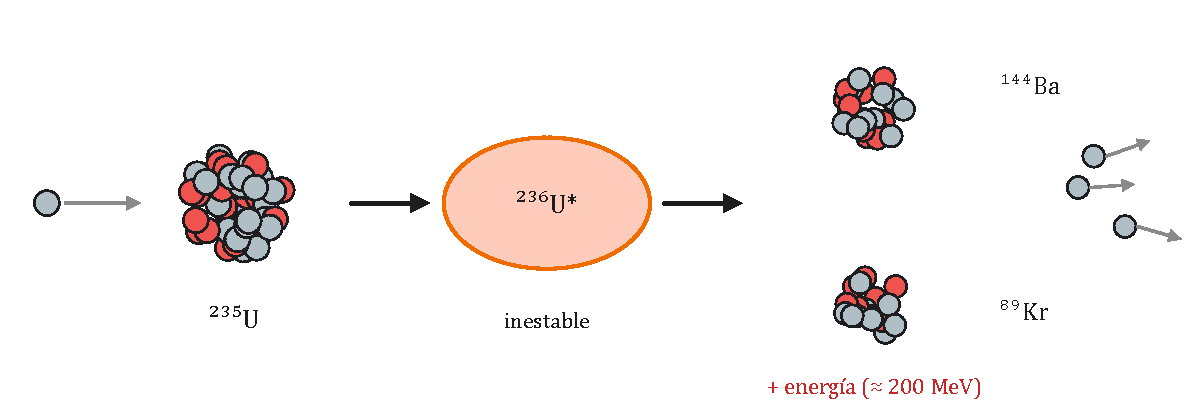
\includegraphics[width=0.85\linewidth]{images/UD8/fision}
    \caption{Fisión del uranio-235 inducida por un neutrón lento.}
    \label{fig:nuc-fision}
\end{figure}

\paragraph{Reacción en cadena y masa crítica.} Los neutrones liberados pueden provocar nuevas fisiones, que liberan más neutrones, y así
sucesivamente: es una \azuln{reacción en cadena} (figura~\ref{fig:nuc-cadena}). Para que se mantenga, la muestra tiene que superar una
\azuln{masa crítica}; si es más pequeña, demasiados neutrones escapan por la superficie.

\begin{figure}[H]
    \centering
    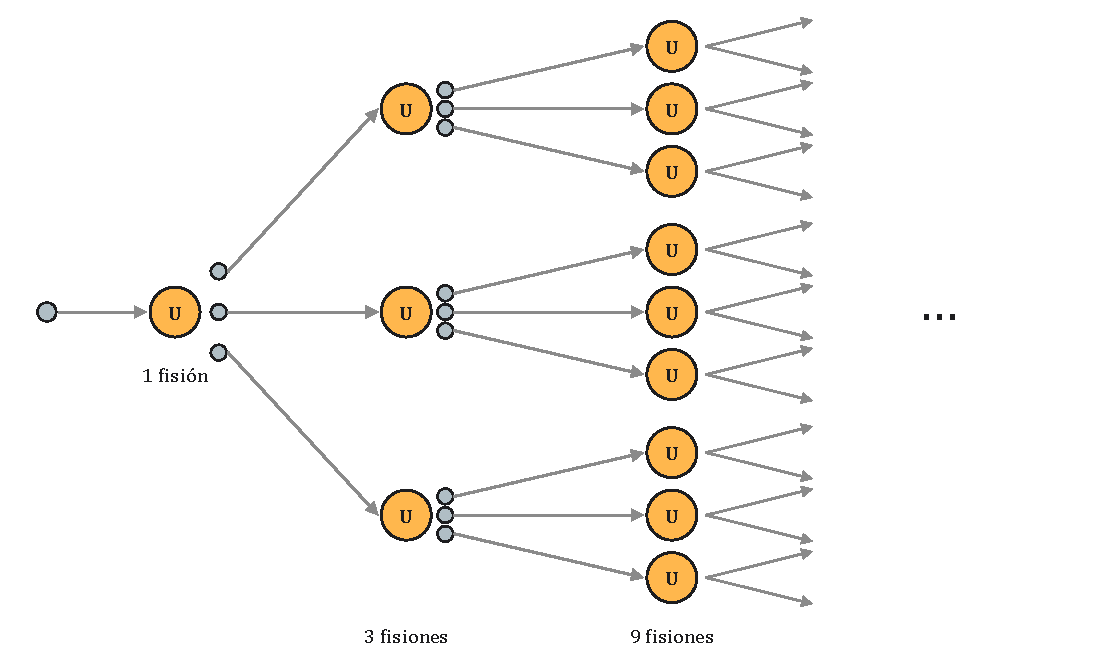
\includegraphics[width=0.66\linewidth]{images/UD8/cadena}
    \caption{Reacción en cadena: si cada fisión provoca, de media, más de una fisión nueva, el número de fisiones crece exponencialmente.}
    \label{fig:nuc-cadena}
\end{figure}

\paragraph{Reactores nucleares.} En un reactor la reacción en cadena se mantiene controlada, de modo que cada fisión provoca exactamente
otra (figura~\ref{fig:nuc-reactor}). Sus partes principales son:
\begin{itemize}
    \item el \textbf{combustible} (uranio enriquecido en \ch{^{235}U}), en barras;
    \item el \textbf{moderador} (agua, agua pesada o grafito), que frena los neutrones para que provoquen fisiones con más facilidad;
    \item las \textbf{barras de control} (cadmio o boro), que absorben neutrones y regulan la reacción;
    \item el \textbf{refrigerante}, que extrae el calor y lo lleva al generador de vapor; el vapor mueve una turbina unida a un alternador;
    \item el \textbf{reflector} y el \textbf{blindaje}, que devuelven los neutrones al núcleo y protegen de la radiación.
\end{itemize}
Si la reacción no se controla y se libera toda la energía en un instante, se tiene una bomba atómica.

\begin{figure}[H]
    \centering
    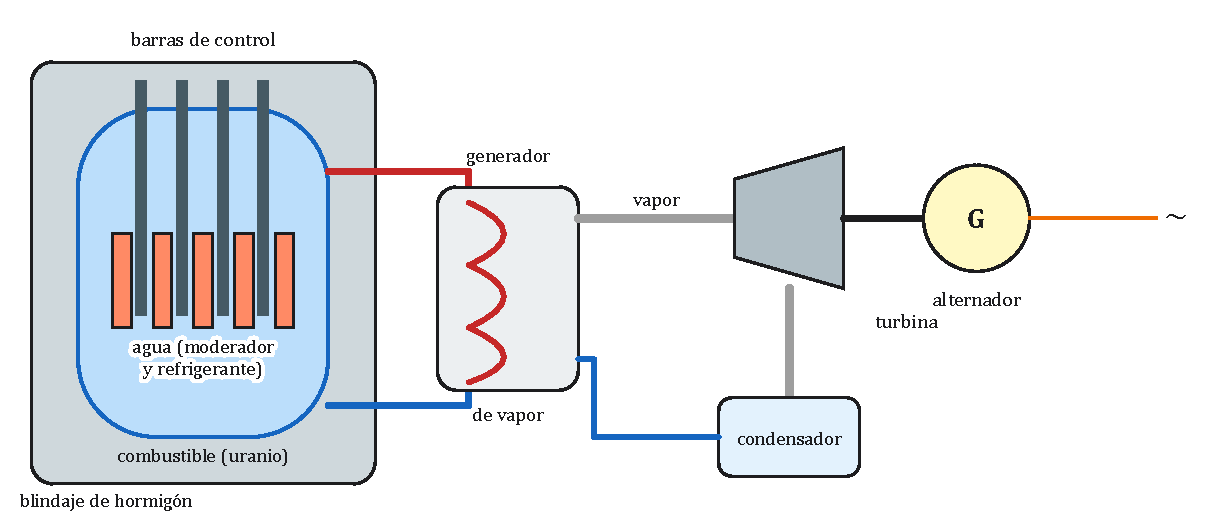
\includegraphics[width=0.85\linewidth]{images/UD8/reactor}
    \caption{Esquema simplificado de una central nuclear de agua a presión.}
    \label{fig:nuc-reactor}
\end{figure}

\begin{exercise}
    En la fisión \(\ch{^{235}_{92}U + ^1_0n -> ^{94}_{38}Sr + ^{140}_{54}Xe + 2 ^1_0n}\), calcula la energía liberada por cada núcleo
    fisionado y la masa de uranio-235 que consume en una hora una central de \qty{3000}{\mega\watt} térmicos. Masas: U-235,
    \qty{235.0439}{u}; Sr-94, \qty{93.9154}{u}; Xe-140, \qty{139.9216}{u}; neutrón, \qty{1.0087}{u}.
    \begin{solu}
        \(\Delta m = 235{,}0439 + 1{,}0087 - 93{,}9154 - 139{,}9216 - 2\cdot 1{,}0087 = \qty{0.1982}{u}\);
        \(Q = 0{,}1982\cdot 931{,}5 = \textcolor{red}{\qty{184.6}{\mega\electronvolt}}\).

        \textcolor{blue}{Energía en una hora: \(3\cdot 10^9\cdot 3600 = \qty{1.08e13}{\joule}\); núcleos: \(\dfrac{1{,}08\cdot 10^{13}}{184{,}6\cdot 1{,}6\cdot 10^{-13}} = \num{3.66e23}\).}
        \(m = \dfrac{3{,}66\cdot 10^{23}}{6{,}022\cdot 10^{23}}\cdot 235 = \textcolor{red}{\qty{143}{\g}}\) \textcolor{blue}{(una central de carbón quemaría más de 1000 toneladas).}
    \end{solu}
\end{exercise}

\subsection{Fusión nuclear}\label{subsec:nuc-fusion}

La \rojon{fusión} es la unión de dos núcleos ligeros para formar uno más pesado. Por ejemplo, la de deuterio y tritio
(figura~\ref{fig:nuc-fusion}):
\[ \ch{^2_1H + ^3_1H -> ^4_2He + ^1_0n} \qquad Q = \qty{17.6}{\mega\electronvolt} \]
Por gramo de combustible libera unas cuatro veces más energía que la fisión. Es la fuente de energía de las estrellas: el Sol fusiona
cada segundo unos 600 millones de toneladas de hidrógeno en helio.

\begin{figure}[H]
    \centering
    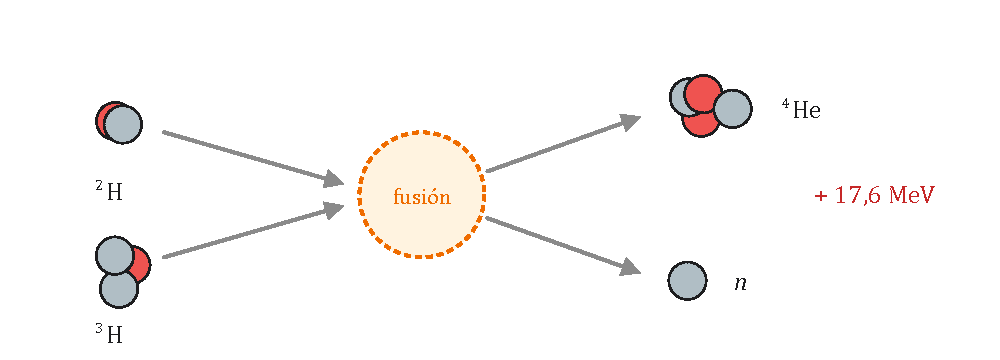
\includegraphics[width=0.66\linewidth]{images/UD8/fusion}
    \caption{Fusión de deuterio y tritio.}
    \label{fig:nuc-fusion}
\end{figure}

Para que dos núcleos se fusionen tienen que vencer su repulsión eléctrica, lo que exige temperaturas de unos cien millones de grados. A
esas temperaturas la materia es un \azuln{plasma} (núcleos y electrones separados) que ningún recipiente puede contener. Se investigan dos
formas de confinarlo: el \emph{confinamiento magnético}, con campos magnéticos intensos en reactores de tipo tokamak (como el proyecto
internacional ITER), y el \emph{confinamiento inercial}, comprimiendo pequeñas cápsulas de combustible con láseres muy potentes.

\begin{remark}
    \textbf{Ventajas de la fusión}: combustible casi inagotable (el deuterio se extrae del agua del mar y el tritio se obtiene del litio),
    no produce residuos radiactivos de larga duración y no hay riesgo de reacción descontrolada. \textbf{Inconvenientes}: todavía no se ha
    conseguido producir más energía de la que se consume de forma sostenida; los neutrones vuelven radiactivos los materiales del reactor,
    y las instalaciones son enormemente caras y complejas.
\end{remark}

\section{Radiactividad artificial y aplicaciones}\label{sec:nuc-aplicaciones}

En 1934, Irène Curie y Frédéric Joliot bombardearon aluminio con partículas alfa y obtuvieron un isótopo radiactivo del fósforo que no
existe en la naturaleza:
\[ \ch{^{27}_{13}Al + ^4_2He -> ^{30}_{15}P + ^1_0n} \qquad\qquad \ch{^{30}_{15}P -> ^{30}_{14}Si + ^0_{1}e} \]
Era la primera \textbf{radiactividad artificial}, y en ella aparece la emisión de positrones (\(\beta^+\)). Hoy los
\azuln{radioisótopos} se fabrican sobre todo en reactores, bombardeando núcleos estables con neutrones, y tienen muchas aplicaciones:

\begin{table}[H]
    \centering
    \caption{Aplicaciones de algunos radioisótopos}
    \vspace{-5pt}
    \begin{tabular}{@{}lL{10.4cm}@{}}
        \toprule
        \textbf{Isótopo} & \textbf{Aplicación} \\
        \midrule
        Yodo-131 & Diagnóstico y tratamiento de enfermedades del tiroides \\[3pt]
        Cobalto-60 & Radioterapia contra el cáncer; esterilización de material quirúrgico y de alimentos \\[3pt]
        Tecnecio-99m & Gammagrafías (el isótopo más usado en medicina nuclear) \\[3pt]
        Flúor-18 & Tomografía por emisión de positrones (PET) \\[3pt]
        Carbono-14 & Datación de restos orgánicos \\[3pt]
        Hidrógeno-3 (tritio) & Trazador en estudios del agua; señales luminosas \\[3pt]
        Fósforo-32 & Trazador en biología y agricultura (absorción de fertilizantes) \\[3pt]
        Americio-241 & Detectores de humo \\
        \bottomrule
    \end{tabular}
    \label{tab:nuc-aplicaciones}
\end{table}

\paragraph{Efectos biológicos y dosis.} Las radiaciones ionizantes pueden dañar las células y el ADN. Para medir sus efectos se usan:
\begin{itemize}
    \item la \azuln{dosis absorbida}, energía absorbida por kilogramo de tejido, medida en \emph{grays} (\(\qty{1}{Gy} = \qty{1}{\joule\per\kg}\));
    \item la \azuln{dosis equivalente}, que multiplica la anterior por un factor que tiene en cuenta el tipo de radiación (1 para \(\beta\)
    y \(\gamma\), 20 para \(\alpha\)), medida en \emph{sieverts} (\unit{Sv}).
\end{itemize}
Recibimos de forma natural (rayos cósmicos, radón del suelo, alimentos) unos \qty{2.4}{mSv} al año; una radiografía de tórax supone unos
\qty{0.1}{mSv}. El límite recomendado para la población, además de la radiación natural, es de \qty{1}{mSv} al año. Para protegerse de una
fuente radiactiva hay tres reglas: \textbf{distancia}, \textbf{tiempo} de exposición corto y \textbf{blindaje}.

\section{Resumen de fórmulas}\label{sec:nuc-resumen}

\begin{table}[H]
    \centering
    \caption{Fórmulas principales de la física nuclear}
    \vspace{-5pt}
    \begin{tabular}{@{}lL{10cm}@{}}
        \toprule
        \textbf{Magnitud} & \textbf{Expresión} \\
        \midrule
        Núcleo & \(A = Z + N\), \quad \(R = r_0 A^{1/3}\), \quad \(r_0 = \qty{1.2e-15}{\m}\) \\[3pt]
        Masa y energía & \(E = mc^2\), \quad \(\qty{1}{u} = \qty{1.66e-27}{\kg} \equiv \qty{931.5}{\mega\electronvolt}\) \\[3pt]
        Energía de enlace & \(\Delta m = Z m_p + N m_n - m_{\text{núcleo}}\), \quad \(E_e = \Delta m\,c^2\), \quad \(E_e/A\) \\[3pt]
        Desplazamientos & \(\alpha\): \(Z - 2\), \(A - 4\); \quad \(\beta^-\): \(Z + 1\); \quad \(\beta^+\): \(Z - 1\); \quad \(\gamma\): sin cambio \\[3pt]
        Desintegración & \(N = N_0 e^{-\lambda t}\), \quad \(A = \lambda N = A_0 e^{-\lambda t}\) \\[3pt]
        Período y vida media & \(T_{1/2} = \ln 2/\lambda\), \quad \(\tau = 1/\lambda\) \\[3pt]
        Energía de una reacción & \(Q = (\sum m_{\text{reactivos}} - \sum m_{\text{productos}})\,c^2\) \\
        \bottomrule
    \end{tabular}
    \label{tab:nuc-resumen}
\end{table}

\section{Prácticas}\label{sec:nuc-practicas}

\subsection{Práctica 1: simulación de la desintegración con dados}\label{subsec:nuc-practica-dados}

\textbf{Objetivo.} Comprobar el carácter aleatorio de la desintegración y obtener la ley exponencial y el período de semidesintegración.

\textbf{Material.} Unos 100 dados (o monedas, o caramelos con una cara marcada) y una caja.

\textbf{Procedimiento.}
\begin{enumerate}[label=\numberballmDarkTeal]
    \item Cada dado es un «núcleo». Lánzalos todos: los que saquen un 6 se han «desintegrado» y se retiran. Anota cuántos quedan.
    \item Repite con los que quedan hasta que queden muy pocos. Cada lanzamiento es una unidad de tiempo.
    \item Junta los datos de toda la clase para tener más núcleos.
\end{enumerate}

\textbf{Cálculos y cuestiones.}
\begin{enumerate}[label=\letraminuscula]
    \item Representa \(N\) frente al número de lanzamientos y \(\ln N\) frente al número de lanzamientos. ¿Qué forma tienen las gráficas?
    \item La pendiente de la segunda es \(-\lambda\). Compárala con la probabilidad de sacar un 6 (\(1/6\)) y calcula \(T_{1/2}\).
    \item ¿Puedes predecir qué dado concreto se «desintegrará» en el siguiente lanzamiento? ¿Y cuántos lo harán, aproximadamente?
\end{enumerate}

\subsection{Práctica 2: radiactividad ambiental}\label{subsec:nuc-practica-contador}

\textbf{Objetivo.} Medir la radiación de fondo y comprobar cómo varía con la distancia y con el blindaje.

\textbf{Material.} Contador Geiger (o la aplicación de un móvil con un detector adaptado), fuentes de muy baja actividad de uso escolar o
materiales naturalmente radiactivos (fertilizante de potasio, sal sin sodio, granito), láminas de papel, aluminio y plomo.

\textbf{Procedimiento.}
\begin{enumerate}[label=\numberballmDarkTeal]
    \item Mide el número de cuentas por minuto sin ninguna fuente, varias veces: es la radiación de fondo.
    \item Coloca la muestra a distintas distancias del detector y mide las cuentas (restando el fondo).
    \item Interpón papel, aluminio y plomo entre la muestra y el detector y anota cómo cambian las cuentas.
\end{enumerate}

\textbf{Cuestiones.}
\begin{enumerate}[label=\letraminuscula]
    \item ¿Por qué el número de cuentas no es exactamente igual en medidas repetidas?
    \item ¿Cómo varían las cuentas con la distancia? ¿Se parece a \(1/r^2\)?
    \item A partir de los blindajes, ¿qué tipo de radiación emite la muestra? Relaciónalo con las tres reglas de protección.
\end{enumerate}
